\documentclass[paper=a4, fontsize=11pt, parskip=full]{scrartcl} % A4 paper and 11pt font size
\usepackage{epsfig}
\usepackage[T1]{fontenc} % Use 8-bit encoding that has 256 glyphs
\usepackage{fourier} % Use the Adobe Utopia font for the document - comment this line to return to the LaTeX default
\usepackage[english]{babel} % English language/hyphenation
\usepackage{amsmath,amsfonts,amsthm,amssymb} % Math packages

\usepackage{sectsty} % Allows customizing section commands
\allsectionsfont{\centering \normalfont\scshape} % Make all sections centered, the default font and small caps

\usepackage{xspace}

\usepackage{fancyhdr} % Custom headers and footers
\pagestyle{fancyplain} % Makes all pages in the document conform to the custom headers and footers
\fancyhead{} % No page header - if you want one, create it in the same way as the footers below
\fancyfoot[L]{} % Empty left footer
\fancyfoot[C]{} % Empty center footer
\fancyfoot[R]{\thepage} % Page numbering for right footer
\renewcommand{\headrulewidth}{0pt} % Remove header underlines
\renewcommand{\footrulewidth}{0pt} % Remove footer underlines
\setlength{\headheight}{13.6pt} % Customize the height of the header

\setlength\parindent{5pt} %minor paragraph indenting

\usepackage{array,booktabs}% for tables



%Cube-related variables
\newcommand*{\A}{\fontfamily{pcr}\selectfont} %for the algorithm type face
\newcommand{\2}{\ensuremath{^2}} %for "twice" in algorithms
\newcommand*\p[2]{\ensuremath{p={}^{#1}\!/_{#2}}}  %for the probabilities
\newcommand*{\nl}{\newline}
\newcommand{\faceWidth}{1.2in} %side of the Rubick's cube faces

\usepackage[normalem]{ulem}

%\newcommand*{\R}{$\mathbb{R}$\xspace}
\newcommand*{\R}{$\mathbb{R}$\xspace}
\newcommand*{\Rp}{$\dot{\mathbb{R}}$\xspace}
\newcommand*{\F}{$\mathbb{F}$\xspace}
\newcommand*{\Fp}{$\dot{\mathbb{F}}$\xspace}
\newcommand*{\U}{$\mathbb{U}$\xspace}
\newcommand*{\Up}{$\dot{\mathbb{U}}$\xspace}



%Where the graphics lie
\usepackage{graphicx}
\graphicspath{
  {Figures/OLL_1/} 
  {Figures/OLL_2/}
  {Figures/PLL_edges/} 
  {Figures/PLL_corners/} 
  {Figures/PLL/} 
  {Figures/notation/}
}

%----------------------------------------------------------------------------------------
%	TITLE SECTION
%----------------------------------------------------------------------------------------

\newcommand{\horrule}[1]{\rule{\linewidth}{#1}} % Create horizontal rule command with 1 argument of height

\title{	
\normalfont \normalsize 
%\textsc{Rob Campbell} \\ [25pt]
\horrule{0.5pt} \\[0.4cm] % Thin top horizontal rule
\huge The Fridrich Method -- Last Layer \\ % The assignment title
\horrule{2pt} \\[0.5cm] % Thick bottom horizontal rule
}

%\author{Rob Campbell} % Your name

\date{\normalsize\today} % Today's date or a custom date





\begin{document}

\maketitle % Print the title



%----------------------------------------------------------------------------------------
%	DOCUMENT BEGINS
%----------------------------------------------------------------------------------------

\section{Breaking down the Fridrich method}

The Fridrich method, also known as CFOP\footnote{\textbf{C}ross, \textbf{F}irst two layers
\textbf{O}rient last layer, \textbf{P}ermute last layer}, is a popular collection of 
algorithms used in speed cubing. Whilst not commonly considered a beginner's method,
CFOP can become so if approached correctly. The purpose of this guide is to get you using
CFOP early on in your cubing adventures. To use this guide, however, you will need to be 
able to solve the first two layers intuitively. If you cannot yet do this, I suggest you 
work through the following steps: 1) Learn to solve the white (for now) cross on the bottom; 
2) Learn to solve the corners of the first layer on the bottom; 3) Learn to intuitively solve 
the first two layers. 
There are good Youtube videos out there to help you achieve those three steps. I like the Paradox Cubing videos (e.g. \texttt{https://www.youtube.com/watch?v=IT5BPHEZGJE}), but others will also work.

After the first two layers, you are faced with learning quite a few algorithms if you want to 
solve the cube using CFOP. Completing the cube is done in two stages: \textbf{o}rienting the cubies on the 
\textbf{l}ast \textbf{l}ayer (OLL) so that all their yellow faces point up towards you, then 
\textbf{p}ermuting the cubies of the \textbf{l}ast \textbf{l}ayer until
they are in the correct positions (PLL). Ideally, this is done in two steps with one algorithm used for
each step. The tricky thing is that there are 57 algorithms for OLL and 21 
for PLL. However you do not need to learn all these algorithms in order to solve the cube with 
CFOP. 

There is the well-known trick of breaking down OLL into two steps: so-called `two look OLL.' 
This reduces the algorithm count to 9 or 10 for this step (Figs.~\ref{OLL1} \& \ref{OLL2}). 
In addition, you can solve the cube with only 2 PLL algorithms: permuting three edges clockwise and permuting three corners clockwise. 
Of course you'll be much slower this way, since you'll need to execute these algorithms several times. 
However, you will have a solved cube and this is a major confidence boost when you're starting out. 
Every PLL algorithm you add from this point will only serve to make you faster. Furthermore, many of 
the algorithms you will need to learn are closely inter-related. For instance, the anti-clockwise versions 
of the corner and edge permutations are simply the clockwise versions run backwards. The purpose
of this guide to help you navigate the algorithm maze.

\subsection{This guide}
This guide presents my favourite algorithms for two-look OLL and PLL. The algorithm choices are 
biased because I solve one handed (left hand). There are minor changes to the conventional 
notation which I made in order to improve readability. The notation is described graphically 
in Section~\ref{sec:notation}. 

In the algorithms I have added spaces to aid visual `chunking' (readability). This is similar
to the use of brackets and/or colours which other guides use. I prefer to avoid using multiple 
colours in algorithms as I find it distracting. Similarly, over-use of brackets clutters 
algorithms and reduces readability. I have used brackets in rare cases where one or more motifs
repeat themselves in the same algorithm. 


\clearpage
\subsection{Orienting the last layer}
\label(OLL)
Tables~\ref{OLL1} and \ref{OLL2} show the algorithms required for two-look OLL. In these tables, 
and others in this guide, the caption at the top summarises the goal the of the moves or provides 
useful information. 


\begin{table}[ht]
  \centering
  \caption{\textit{OLL, first look.} The goal here is to make a yellow cross.
  If you don't wish to learn the algorithm for case C, just execute A followed by B. $p$
  is the probability of finding the cube in the configuration shown.}
  \renewcommand{\arraystretch}{1.5}% Spread rows out...
  \begin{tabular}{>{\centering}m{1.2in} >{}m{1.8in} >{\centering}m{1.2in} >{}m{1.8in}}
    \toprule
    Configuration & Algorithm & Configuration & Algorithm \\
    \midrule

    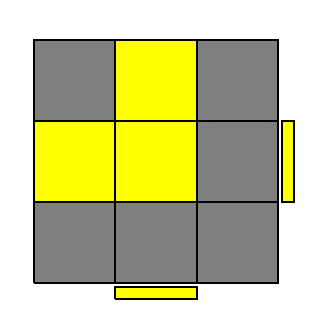
\includegraphics[width=\faceWidth]{OLL_1_1.eps}  & Case A. \p{1}{2}\nl\nl 
    {\A F UR \.{U}\.{R} \.{F} } & 

    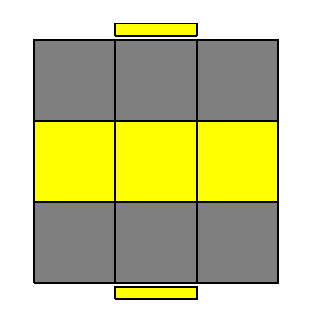
\includegraphics[width=\faceWidth]{OLL_1_2.eps}  & Case B. \p{1}{4}\nl\nl 
    {\A F RU \.{R}\.{U} \.{F} } \\

    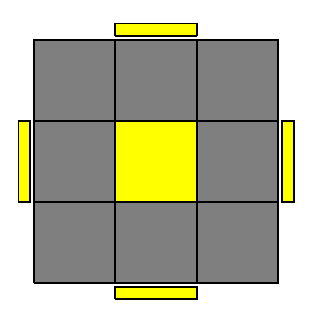
\includegraphics[width=\faceWidth]{OLL_1_3.eps}  & Case C. \p{1}{8}\nl\nl 
    {\A R\.UR\2\.D  r\.U\.r DR\2 U\.R}  & 
   
    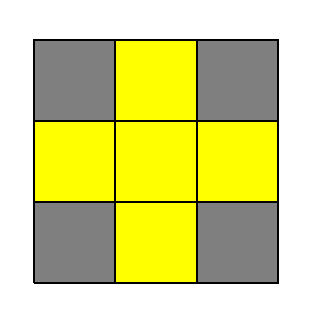
\includegraphics[width=\faceWidth]{OLL_1_4.eps}  & Case D. \p{1}{8}\nl\nl 
    {\A Solved } \\

    \bottomrule
  \label{OLL1}
  \end{tabular}
\end{table}


\clearpage

\begin{table}[ht]
  \centering

  \caption{\textit{OLL, second look.} From a solved state (Case H), executing the algorithm for 
  case Case A takes you to case Case B and vice versa (A$\longleftrightarrow$B). Similarly,
  E$\longleftrightarrow$F. Executing Case G takes you to Case F. The algorithms for Cases C and D 
  rotate the corner pieces, so executing one of these algorithms twice from a solved 
  face returns the cube to a solved face. This stuff is worth knowing because it provides
  a means for practice.}
  \renewcommand{\arraystretch}{1.5}% Spread rows out...
  \begin{tabular}{>{\centering}m{1.2in} >{}m{1.8in} >{\centering}m{1.2in} >{}m{1.8in}}
    \toprule
    Configuration & Algorithm & Configuration & Algorithm \\
    \midrule

    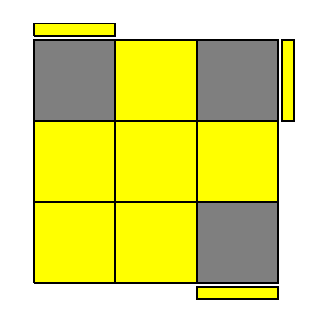
\includegraphics[width=\faceWidth]{OLL_2_1.eps}  & Case A. \p{4}{27}\nl\nl 
    {\A RU \.{R} UR U\2\.{R} } & 

    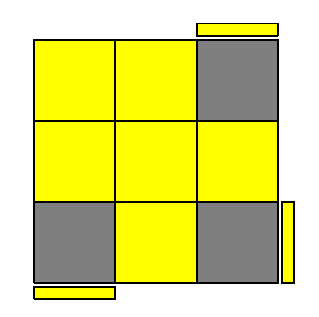
\includegraphics[width=\faceWidth]{OLL_2_2.eps}  & Case B. \p{4}{27}\nl\nl 
    {\A \.{R}\.{U} R \.{U}\.{R} U\2R} \\

    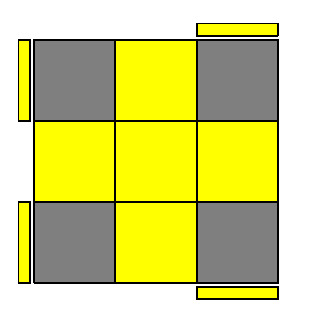
\includegraphics[width=\faceWidth]{OLL_2_3.eps}  & Case C. \p{4}{27}\nl\nl 
    {\A R U\2R\2 \.{U}R\2 \.{U}R\2 U\2R}  & 

    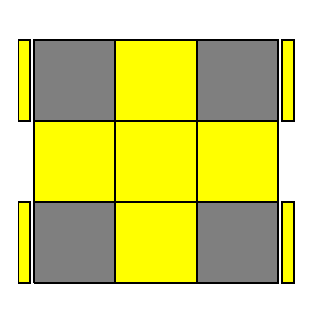
\includegraphics[width=\faceWidth]{OLL_2_4.eps}  & Case D. \p{2}{27}\nl\nl 
    {\A RU\.{R}U R\.{U}\.{R}U RU\2\.{R} } \\

    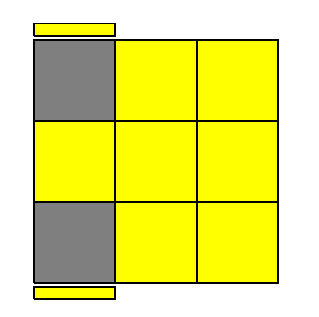
\includegraphics[width=\faceWidth]{OLL_2_5.eps}  & Case E. \p{4}{27}\nl\nl 
    {\A r U\.{R}\.{U} \.{r} FR\.{F}} & 

    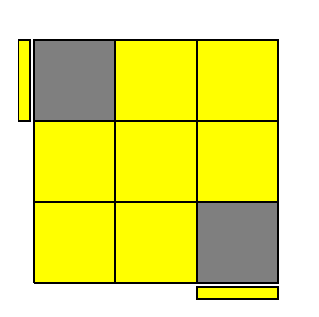
\includegraphics[width=\faceWidth]{OLL_2_6.eps}  & Case F. \p{4}{27}\nl\nl 
    {\A \.{F} r U\.{R}\.{U} \.{r} FR }   \\

    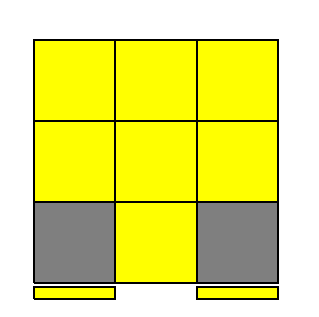
\includegraphics[width=\faceWidth]{OLL_2_7.eps}  & Case G. \p{4}{27}\nl\nl 
    {\A R\2D \.{R}U\2 R\.{D} \.{R}U\2\.{R} }  \nl
    {\A RU\.{R}U R U\2R\2 \.{U}R\.{U}\.{R} U\2R} &

    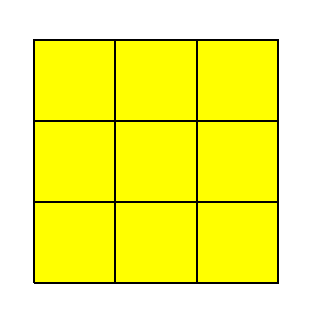
\includegraphics[width=\faceWidth]{OLL_2_8.eps}  & Case H. \p{1}{27}\nl\nl 
    {\A Solved } \\


    \bottomrule

  \end{tabular}
  \label{OLL2}
\end{table}

\clearpage

\section{PLL: the least you need}
The tables below describe the complete PLL procedure. The edge colors are purely illustrative; 
in other words, if you have 
Case Ua (Table~\ref{PLL_edges}) it will manifest with a solved blue side only one quarter of the 
time. It could also be a solved red, green, or orange side. 

Although there are 21 algorithms below, in theory you can get away with learning only one edge 
permutation algorithm (Table~\ref{PLL_edges} Ua or Ub) and one corner permutation 
algorithm (Table~\ref{PLL_corners} Aa or Ab). This will be sufficient solve PLL, but it will be 
slow. For instance, if you have a situation where two edges are solved, you will have to run the 
edge permutation algorithm multiple times. Once to move one solved edge but leave the 
other one in place, then at least one more time after you've figured out which edge is now 
correct and which three edges now need to move. The after you've done all that you will need to 
permute the corners. Whilst this is more time consuming, it does mean that once you've learned 
this minimal set of algorithms you can solve the cube. So you'll be able to practice going 
from scrambled to solved states relatively soon. This allows you to work on the whole process, 
and add more PLL algorithms in time. 

\begin{table}[ht]
  \centering
  \caption{\textit{PLL: edge permutations}. Cases Ua \& Ub are essentially the same: the 
  Ua algorithm is just the Ub algorithm run backwards. You could solve the Ua case by running the algorithm for Ub twice.
  Cases Z and H have double-headed arrows, indicating that these pieces are swapped. 
  If your run withr Z or H twice you will end up in the original configuration. }
  \renewcommand{\arraystretch}{1.5}% Spread rows out...
  \begin{tabular}{>{\centering}m{1.2in} >{}m{1.8in} >{\centering}m{1.2in} >{}m{1.8in}}
    \toprule
    Configuration & Algorithm & Configuration & Algorithm \\
    \midrule

    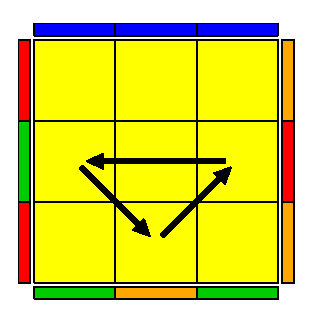
\includegraphics[width=\faceWidth]{PLL_edges_1.eps}  & Case Ua. \p{1}{18}\nl\nl 
    {\A R\.{U}R UR UR \.{U}\.{R}\.{U} R\2}  & 

    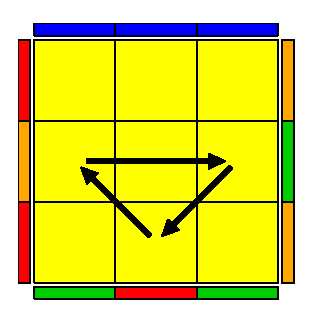
\includegraphics[width=\faceWidth]{PLL_edges_2.eps}  & Case Ub. \p{1}{18}\nl\nl 
    {\A R\2 URU \.{R}\.{U} \.{R}\.{U} \.{R}U\.{R} } \\


    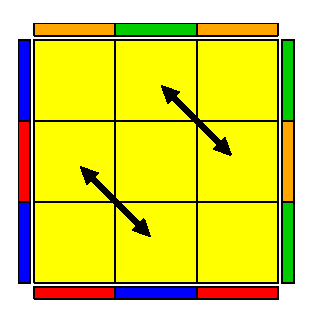
\includegraphics[width=\faceWidth]{PLL_edges_3.eps}  & Case Z. \p{1}{36}\nl\nl 
    {\A \.{R}\.{U}R\.{U} RU R\.{U}\.{R}U RUR\2 \.{U}\.{R}U\2 } &

    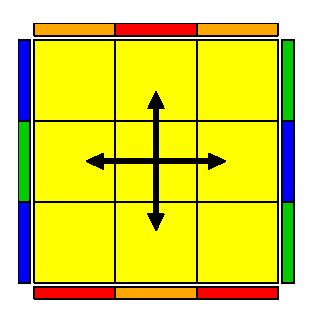
\includegraphics[width=\faceWidth]{PLL_edges_4.eps}  & Case H. \p{1}{72}\nl\nl 
    {\A R\2U\2 R U\2R\2 U\2R\2 U\2 R U\2R\2  } \\

    \bottomrule
  \end{tabular}
  \label{PLL_edges}
\end{table}




\begin{table}[ht]
  \centering
  \caption{\textit{PLL: corner permutations.} Case E is long but repetitive, 
  so not too hard to learn. Since Aa and Ab are inverses of each other, so it's
  easy to learn both. However, since they both just cycle corners in different directions
  you can get away with just Aa or Ab initially if that's what you wish. Overall, learning
  all three corner permutation algorithms is fairly easy.}
  \renewcommand{\arraystretch}{1.5}% Spread rows out...
  \begin{tabular}{>{\centering}m{1.2in} >{}m{1.8in} >{\centering}m{1.2in} >{}m{1.8in}}
    \toprule
    Configuration & Algorithm & Configuration & Algorithm \\
    \midrule

    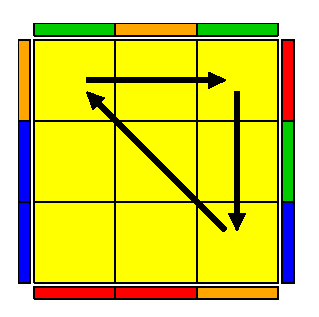
\includegraphics[width=\faceWidth]{PLL_corners_1.eps}  & Case Aa. \p{1}{18}\nl\nl 
    {\A \R \.{R}U\.{R} D\2 R\.{U}\.{R} D\2R\2} & 

    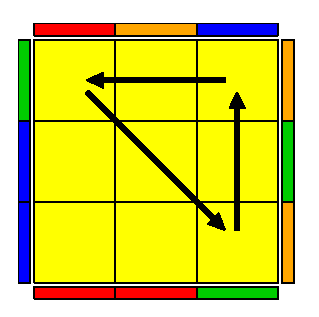
\includegraphics[width=\faceWidth]{PLL_corners_2.eps}  & Case Ab. \p{1}{18}\nl\nl 
    {\A \R R\2D\2 RU\.{R} D\2 R\.{U}R } \\

    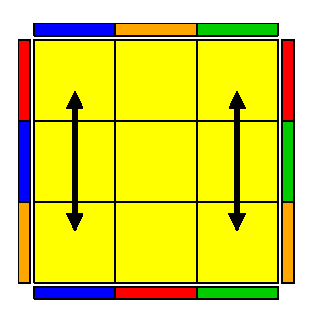
\includegraphics[width=\faceWidth]{PLL_corners_3.eps}  & Case E. \p{1}{36}\nl\nl
    {\A \Rp R\.{U}\.{R} D RU\.{R} \.{D}  RU\.{R} D  R\.{U}\.{R}  \.{D}} &

    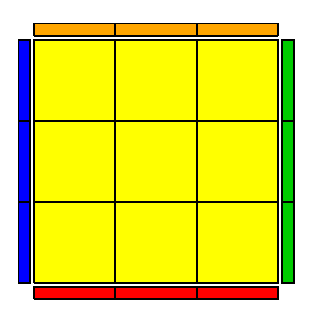
\includegraphics[width=\faceWidth]{PLL_solved.eps}  & \p{1}{72}\nl\nl 
    {\A Solved} \\

    \bottomrule
  \end{tabular}
  \label{PLL_corners}
\end{table}


\begin{table}[ht]
  \centering
  \caption{\textit{PLL: opposite edge and corner switches.} Both of these algorithms 
  switch one pair of opposite edges and one pair of opposite corners. The motifs 
  {\A RU\.{R}\.{U}} and {\A \.{R}\.{U}RU} are just inverses of each other and shared between the 
  two cases, F \& T, shown here. In T it helps to track the F2L pairs to help memorise. Note that 
  the Case F algorithm is almost the same as that for Case V (Fig.~\ref{PLL_diagonal}). }
  \renewcommand{\arraystretch}{1.5}% Spread rows out...
  \begin{tabular}{>{\centering}m{1.2in} >{}m{1.8in} >{\centering}m{1.2in} >{}m{1.8in}}
    \toprule
    Configuration & Algorithm & Configuration & Algorithm \\
    \midrule

    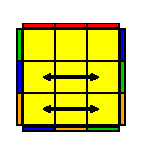
\includegraphics[width=\faceWidth]{PLL_F.eps}  & Case F. \p{1}{18}\nl\nl 
    {\A \.{R}U\2\.{R}\.{d} \.{R}\.{F} R\2\.{U}\.{R}U \.{R}FR\.UF} \nl
    {\A \U \.{R}\.{U}\.{F} RU\.{R}\.{U} \.{R}FR\2\.{U} \.{R}\.{U}RU \.{R}UR} &

    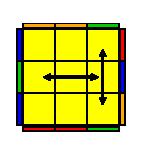
\includegraphics[width=\faceWidth]{PLL_T.eps}  & Case T. \p{1}{18}\nl\nl 
    {\A  RU\.{R}\.{U} \.{R}F R\2\.{U}\.{R} \.{U} RU\.{R}\.{F} } \\

    \bottomrule
  \end{tabular}
  \label{PLL_opposites}
\end{table}

\begin{table}[ht]
  \centering
  \caption{\textit{PLL: swap adjacent corners and an edge pair.} In Case Ja, the {\A \.{R}\R} can 
  be substituted with {\A \.{l}} if you're solving two-handed. Ja presents white side up when 
  solved. Notice that Jb and T (above) are closely related: {\A RU\.{R}\.{F}} is moved to the begin in 
  Jb and the rest is the same as T. Easy! }
  \renewcommand{\arraystretch}{1.5}% Spread rows out...
  \begin{tabular}{>{\centering}m{1.2in} >{}m{1.8in} >{\centering}m{1.2in} >{}m{1.8in}}
    \toprule
    Configuration & Algorithm & Configuration & Algorithm \\
    \midrule

    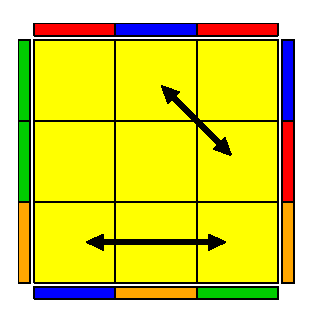
\includegraphics[width=\faceWidth]{PLL_Ra.eps}  & Case Ra. \p{1}{18}\nl\nl 
    {\A RU\2 \.{R}U\2 R\.{B} \.{R}\.{U}RU RB R\2U } & 

    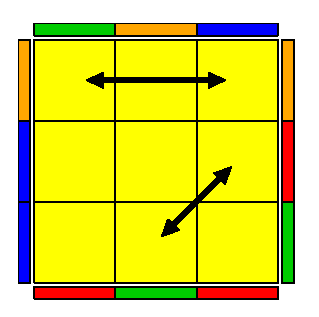
\includegraphics[width=\faceWidth]{PLL_Rb.eps}  & Case Rb. \p{1}{18}\nl\nl 
    {\A  \.{R}U\2RU\2 \.{R}F RU\.{R}\.{U} \.{R}\.{F} R\2\.{U} } \\

    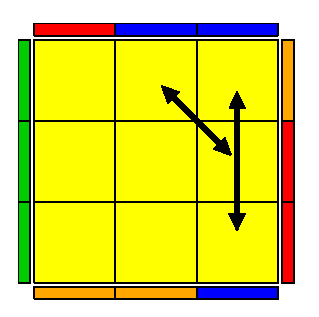
\includegraphics[width=\faceWidth]{PLL_Ja.eps}  & Case Ja. \p{1}{18}\nl\nl 
    {\A \R U\2 \.{r}\.{U} rU\2 \.{R}\R U\.{R}\.{U} R\2} &

    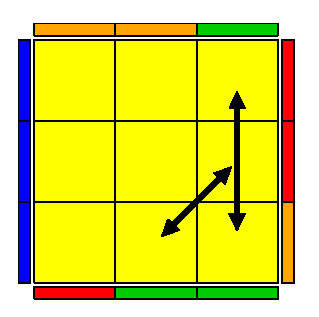
\includegraphics[width=\faceWidth]{PLL_Jb.eps}  & Case Jb. \p{1}{18}\nl\nl 
    {\A  RU\.{R}\.{F} RU\.{R}\.{U} \.{R}F R\2\.{U}\.{R} \.{U} } \\

    \bottomrule
  \end{tabular}
  \label{PLL_adjacent}
\end{table}

\begin{table}[ht]
  \centering
  \caption{\textit{PLL: swap diagonal corners and an edge pair.} Note that in Nb a
  portion of the algorithm in square brackets is repeated twice (this is what $\cdot2$ means). These algorithms are also inverses
  of each other since the two cases are mirror images. Follow the F2L pairs in Y.}
  \renewcommand{\arraystretch}{1.5}% Spread rows out...
  \begin{tabular}{>{\centering}m{1.2in} >{}m{1.8in} >{\centering}m{1.2in} >{}m{1.8in}}
    \toprule
    Configuration & Algorithm & Configuration & Algorithm \\
    \midrule

    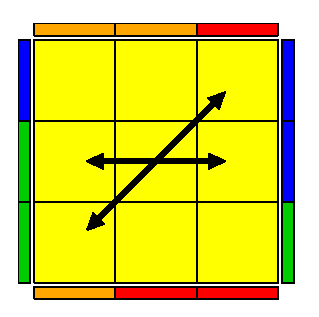
\includegraphics[width=\faceWidth]{PLL_Na.eps}  & Case Na. \p{1}{72}\nl\nl 
    {\A RU\.{R} URU  \.{R}\.{F}R  U  \.{R}\.{U}\.{R}  FR\2 \.{U}\.{R} U2 R\.{U}\.{R}} &


    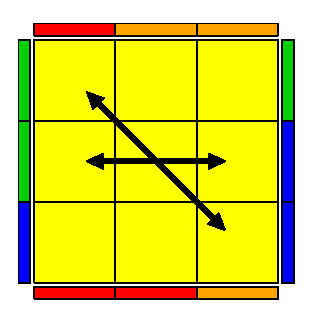
\includegraphics[width=\faceWidth]{PLL_Nb.eps}  & Case Nb. \p{1}{72}\nl\nl 
    {\A  [\.{R}U \.{L}U\2 R\.{U} L]$\cdot2$ U } \\

    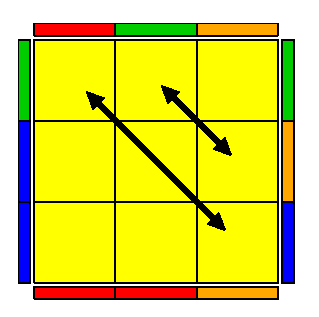
\includegraphics[width=\faceWidth]{PLL_V.eps}  & Case V. \p{1}{18}\nl\nl 
    {\A \.{R}U\.{R}\.{d} \.{R}\.{F} R\2\.{U}\.{R}U \.{R}FRF} & 

    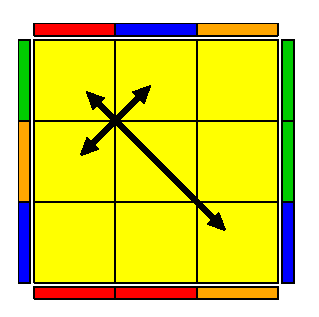
\includegraphics[width=\faceWidth]{PLL_Y.eps}  & Case Y. \p{1}{18}\nl\nl 
    {\A F R\.{U}\.{R} \.{U} RU\.{R}\.{F} RU\.{R}\.{U} \.{R}FR\.{F}} \\

    \bottomrule
  \end{tabular}
  \label{PLL_diagonal}
\end{table}



\begin{table}[ht]
  \centering
  \caption{\textit{PLL: double rotations.} These moves permute both the corners and the edges.
  Running Ga on a solved cube gives you Gb. Similarly Gc and Gd share the same relationship. }
  \renewcommand{\arraystretch}{1.5}% Spread rows out...
  \begin{tabular}{>{\centering}m{1.2in} >{}m{1.8in} >{\centering}m{1.2in} >{}m{1.8in}}
    \toprule
    Configuration & Algorithm & Configuration & Algorithm \\
    \midrule

    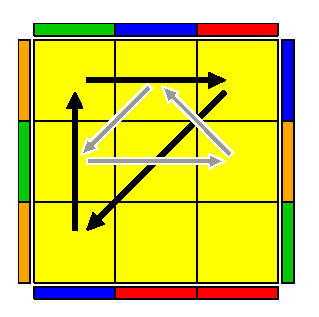
\includegraphics[width=\faceWidth]{PLL_Ga.eps}  & Case Ga. \p{1}{18}\nl\nl 
    {\A R\2u \.{R}U\.{R}\.{U} R\.{u} R\2 \Up \.{R}UR } & 

    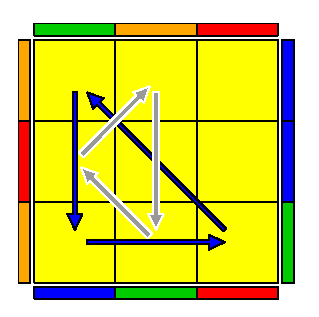
\includegraphics[width=\faceWidth]{PLL_Gb.eps}  & Case Gb. \p{1}{18}\nl\nl 
    {\A \.{R}\.{U}R \U R\2u \.{R}UR\.{U} R\.{u}R\2  } \\


    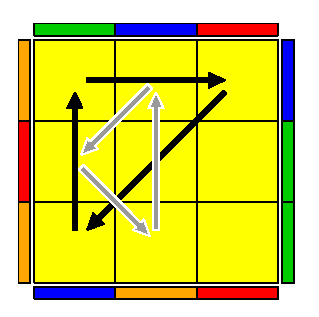
\includegraphics[width=\faceWidth]{PLL_Gd.eps}  & Case Gd. \p{1}{18}\nl\nl 
    {\A RU\.{R} \Up R\2\.{u} R\.{U}\.{R}U \.{R}u R\2 } &

    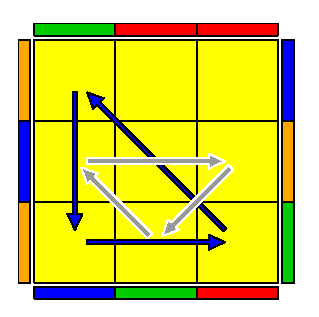
\includegraphics[width=\faceWidth]{PLL_Gc.eps}  & Case Gc. \p{1}{18}\nl\nl 
    {\A R\2\.{u} R\.{U}RU \.{R}u R\2 \U R\.{U}\.{R} } \\


    \bottomrule
  \end{tabular}
  \label{PLL_doubles}
\end{table}




\clearpage
\section{Notation}
\label{sec:notation}
Three different views of a solved cube are shown in Figure~\ref{fig:solved}. The cube is shown in this
orientation for the rest of this section. The red face is the front face, the blue face is the left face, 
the green face is the right face, and the yellow face is the top face. 

Figure~\ref{fig:faceNotation} shows the notation used to the layers 
being manipulated. For example, {\A L} refers to the left face. 
Specifically, in the algorithms above, {\A L} indicates a \textit{clockwise} 
rotation of the left face.  {\A \.{L}} indicates an \textit{anti-clockwise}\footnote{This is obviously
the same as {\A L'}. You can still call it `L-prime' verbally, if you like. The overlying dot just doesn't add the horizontal space taken up by the prime symbol.}
rotation of the left face. For every face, the terms `clockwise'  and `anti-clockwise' 
refer to how the face would appear to rotate if it were facing you. Thus, if you're holding the 
cube with the red face towards you, an {\A R} move will send
 the yellow portion of the {\A R} face away from you whereas an {\A L} move will 
 bring the yellow portion of  the {\A L} face towards you. Finally, {\A L\2} denotes 
 a 180 degree rotation of the {\A L} face. Since the rotation is 180 degrees, it 
 doesn't matter if you execute the motion clockwise or counter-clockwise. There are no 
 rotations of the middle layer alone in this guide. 

\begin{figure}[h]
\centering
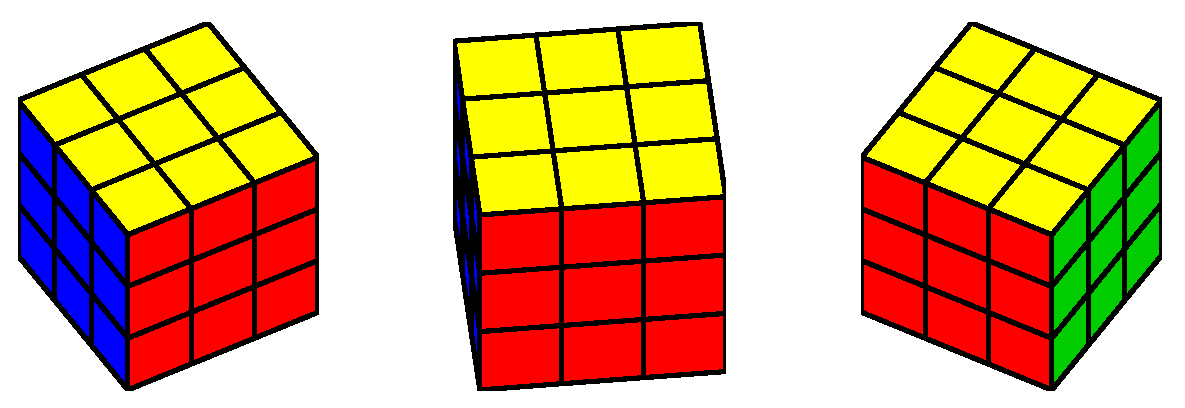
\includegraphics[width=4.5in]{threeViewsOfSolvedCube.eps}
\caption{\textit{Three different views of a solved cube.} The white face is opposite
the yellow face and not shown. The orange face is opposite the red face and not shown. Note that a 
single viewpoint can reveal at most only three of the six faces.}
\label{fig:solved}
\end{figure}


 Hopefully it is pretty obvious how to read Figure~\ref{fig:faceNotation}. Just in case, 
 however, Figure~\ref{fig:exampleTwists} shows four example twists of the cube from
 a solved state. It is straightforward to extrapolate what other moves will look like. 


\clearpage


\begin{figure}
\centering
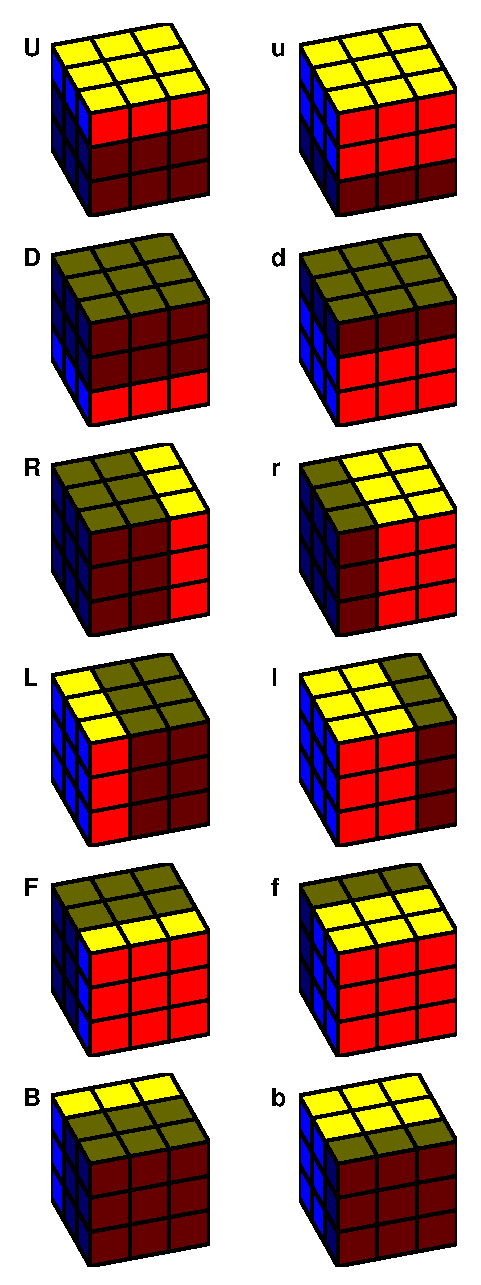
\includegraphics[width=2.5in]{faceNotation.eps}
\caption{\textit{Notation used to describe manipulations of the cube.} The left 
column refers to single layers and the right column to a pair of adjacent layers. The
brighter, highlighted, layers are what are referred to by the character. For example,
{\A U} refers to the \textbf{U}p face. Going down from the top we have: Up, Down,
Right, Left, Front, and Back faces. Lower case letters refer to the 
layer denoted by the upper case letter plus the layer next to it. The dark faces are
those that will stay still and the light faces those that will move.}
\label{fig:faceNotation}
\end{figure}

\clearpage

\begin{figure}[t]
\centering
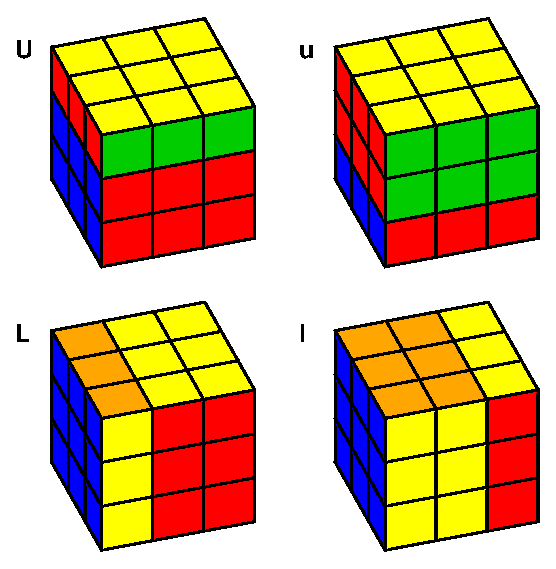
\includegraphics[width=3in]{exampleTwists.eps}
\caption{\textit{Example twists from a solved state.} Four examples showing what the 
cube looks like following single {\A U}, {\A u}, {\A L}, or {\A l} moves from a 
solved state.}
\label{fig:exampleTwists}
\end{figure}

\clearpage

\subsection{Cube rotations}
The final issue concerns rotations of the whole cube. These are sometimes conducted 
in order to make an algorithm easier to perform. The notation is: \R `rotate cube clockwise
with respect to right face', \F `rotate cube clockwise with respect to front face', \U `rotate 
cube clockwise with respect to up face'. Of course all those moves have the counter-clockwise
equivalents \Rp, \Fp, and \Up. All the rotations are shown in Figure~\ref{fig:rotationNotation}. 
There are no 180 degree rotations in this guide, but obviously we would denote these as \R\2, etc...
The rotation notation used here is essentially identical to the existing {\A [r]}, {\A [u]}, and {\A [f]} 
scheme but uses fewer characters. 

\begin{figure}[h]
\centering
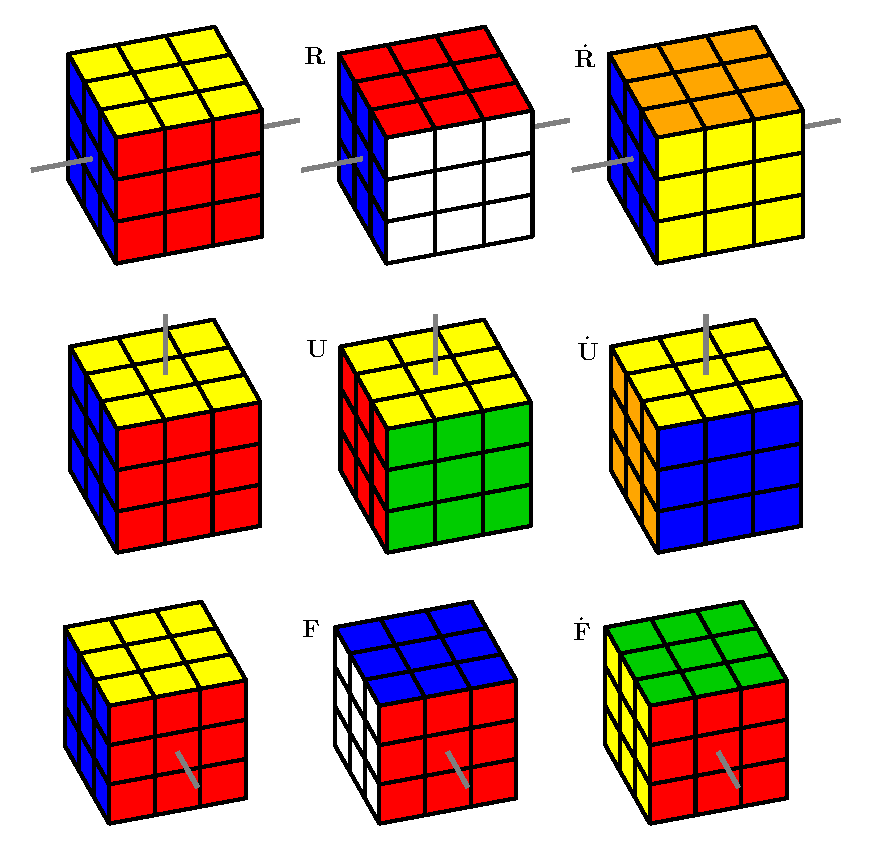
\includegraphics[width=4in]{rotationNotation.eps}
\caption{\textit{Rotation notation.} This guide uses a different notion for cube rotations. 
In case you are familiar with the more common system, in this guide \R={\A x}, \U={\A y}, and
\F={\A z}. Example clockwise and counter-clockwise rotations are shown above for each axis (grey lines). For
example, \R is a clockwise rotation with respect to the right face. The counter-clockwise rotation
is \Rp. The font in this figure differs slightly from the text, but the point holds.}
\label{fig:rotationNotation}
\end{figure}

\clearpage


\thispagestyle{empty}
\renewcommand{\faceWidth}{0.9in} %side of the Rubick's cube faces
\begin{table}[ht]
  \centering
  \caption{Condensed two-look OLL}
  \renewcommand{\arraystretch}{1.5}% Spread rows out...
  \begin{tabular}{>{\centering}m{0.9in} >{}m{1.8in} >{\centering}m{0.9in} >{}m{1.8in}}
    \toprule
    Configuration & Algorithm & Configuration & Algorithm \\
    \midrule

    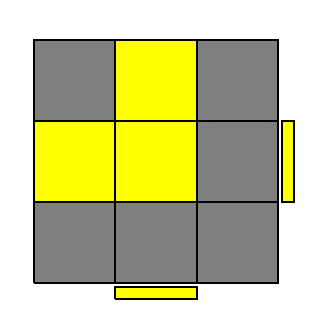
\includegraphics[width=\faceWidth]{OLL_1_1.eps}  & Case A. \p{1}{2}\nl\nl 
    {\A F UR \.{U}\.{R} \.{F} } & 

    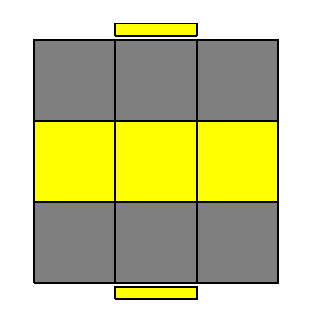
\includegraphics[width=\faceWidth]{OLL_1_2.eps}  & Case B. \p{1}{4}\nl\nl 
    {\A F RU \.{R}\.{U} \.{F} } \\

    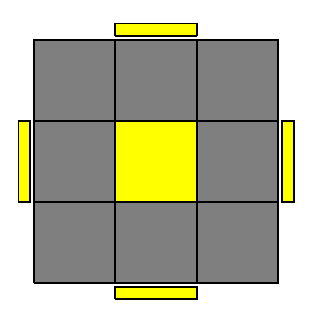
\includegraphics[width=\faceWidth]{OLL_1_3.eps}  & Case C. \p{1}{8}\nl\nl 
    {\A R\.UR\2\.D  r\.U\.r DR\2 U\.R}  & 

    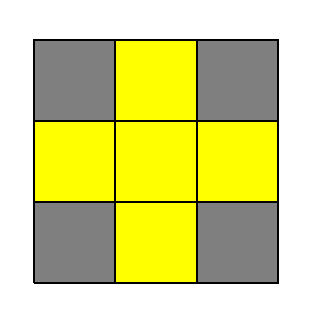
\includegraphics[width=\faceWidth]{OLL_1_4.eps}  & Case D. \p{1}{8}\nl\nl 
    {\A Solved } \\
    \\
    \bottomrule
    \\  
    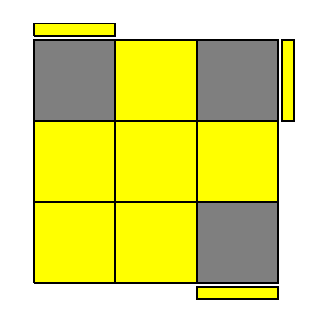
\includegraphics[width=\faceWidth]{OLL_2_1.eps}  & Case A. \p{4}{27}\nl\nl 
    {\A RU \.{R} UR U\2\.{R} } & 

    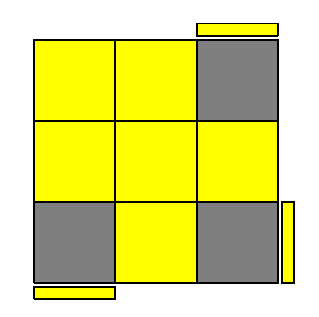
\includegraphics[width=\faceWidth]{OLL_2_2.eps}  & Case B. \p{4}{27}\nl\nl 
    {\A \.{R}\.{U} R \.{U}\.{R} U\2R} \\

    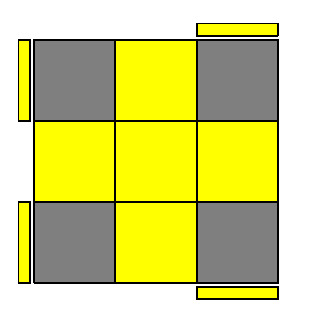
\includegraphics[width=\faceWidth]{OLL_2_3.eps}  & Case C. \p{4}{27}\nl\nl 
    {\A R U\2R\2 \.{U}R\2 \.{U}R\2 U\2R}  & 
   
    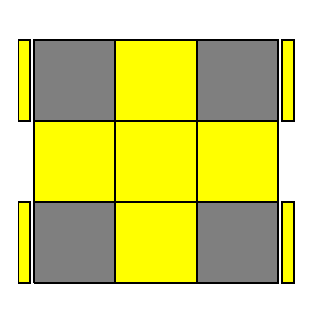
\includegraphics[width=\faceWidth]{OLL_2_4.eps}  & Case D. \p{2}{27}\nl\nl 
    {\A RU\.{R}U R\.{U}\.{R}U RU\2\.{R} } \\

    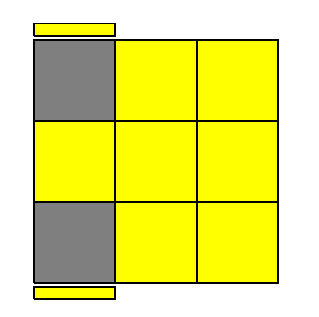
\includegraphics[width=\faceWidth]{OLL_2_5.eps}  & Case E. \p{4}{27}\nl\nl 
    {\A r U\.{R}\.{U} \.{r} FR\.{F}} & 

    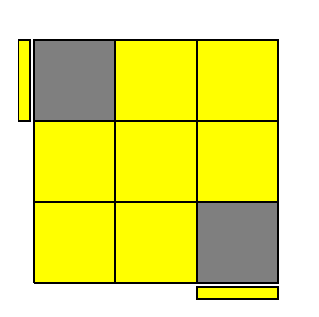
\includegraphics[width=\faceWidth]{OLL_2_6.eps}  & Case F. \p{4}{27}\nl\nl 
    {\A \.{F} r U\.{R}\.{U} \.{r} FR }   \\

    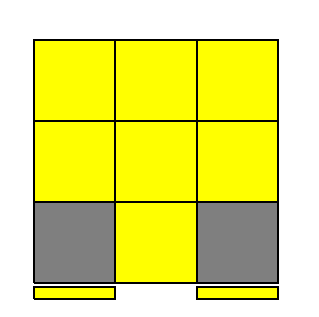
\includegraphics[width=\faceWidth]{OLL_2_7.eps}  & Case G. \p{4}{27}\nl\nl 
    {\A R\2D \.{R}U\2 R\.{D} \.{R}U\2\.{R} }  \nl
    {\A RU\.{R}U R U\2R\2 \.{U}R\.{U}\.{R} U\2R} &

    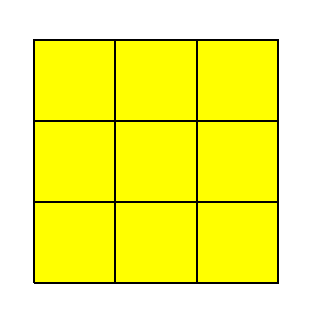
\includegraphics[width=\faceWidth]{OLL_2_8.eps}  & Case H. \p{1}{27}\nl\nl 
    {\A Solved } \\


    \bottomrule
  \end{tabular}
  \label{OLL}
\end{table}





\clearpage

\thispagestyle{empty}

\renewcommand{\faceWidth}{0.75in} 
\begin{table}[ht]
  \centering
  \caption{Condensed PLL.}
  \renewcommand{\arraystretch}{1.5}% Spread rows out...
  \begin{tabular}{>{\centering}m{0.7in} >{}m{2.2in} >{\centering}m{0.7in} >{}m{2in}}
    \toprule
    \includegraphics[width=\faceWidth]{PLL_edges_1.eps}  & Ua. \p{1}{18}\nl
    {\A R\.{U}R UR UR \.{U}\.{R}\.{U} R\2} & 

    \includegraphics[width=\faceWidth]{PLL_edges_2.eps}  & Ub. \p{1}{18}\nl
    {\A R\2 URU \.{R}\.{U} \.{R}\.{U} \.{R}U\.{R} } \\

    \includegraphics[width=\faceWidth]{PLL_edges_3.eps}  & Z. \p{1}{36}\nl
    {\A \.{R}\.{U}R\.{U} RU R\.{U}\.{R}U RUR\2 \.{U}\.{R}U\2 } &

    \includegraphics[width=\faceWidth]{PLL_edges_4.eps}  & H. \p{1}{72}\nl
    {\A R\2U\2 R U\2R\2 U\2R\2 U\2 R U\2R\2  } \\

    \includegraphics[width=\faceWidth]{PLL_corners_1.eps}  & Aa. \p{1}{18}\nl 
    {\A \R \.{R}U\.{R} D\2 R\.{U}\.{R} D\2R\2} & 

    \includegraphics[width=\faceWidth]{PLL_corners_2.eps}  & Ab. \p{1}{18}\nl 
    {\A \R R\2D\2 RU\.{R} D\2 R\.{U}R } \\

    \includegraphics[width=\faceWidth]{PLL_corners_3.eps}  & E. \p{1}{36}\nl
    {\A \Rp R\.{U}\.{R} D RU\.{R} \.{D}  \nl RU\.{R} D  R\.{U}\.{R}  \.{D}} &
    

    \includegraphics[width=\faceWidth]{PLL_solved.eps}  & \p{1}{72}\nl 
    {\A Solved} \\

    \includegraphics[width=\faceWidth]{PLL_F.eps}  & F. \p{1}{18}\nl 
    {\A \.{R}U\2\.{R}\.{d} \.{R}\.{F} R\2\.{U}\.{R}U \.{R}FR\.UF} \nl
    {\A \U \.{R}\.{U}\.{F} RU\.{R}\.{U} \.{R}FR\2\.{U} \.{R}\.{U}RU \.{R}UR} &

    \includegraphics[width=\faceWidth]{PLL_T.eps}  & T. \p{1}{18}\nl 
    {\A  RU\.{R}\.{U} \.{R}F R\2\.{U}\.{R} \.{U} RU\.{R}\.{F} } \\

    \includegraphics[width=\faceWidth]{PLL_Ra.eps}  & Ra. \p{1}{18}\nl 
    {\A RU\2 \.{R}U\2 R\.{B} \.{R}\.{U}RU RB R\2U} & 

    \includegraphics[width=\faceWidth]{PLL_Rb.eps}  & Rb. \p{1}{18}\nl 
    {\A  \.{R}U\2RU\2 \.{R}F RU\.{R}\.{U} \.{R}\.{F} R\2\.{U} } \\

    \includegraphics[width=\faceWidth]{PLL_Ja.eps}  & Ja. \p{1}{18}\nl 
    %{\A F\2 \.{L}\.{U} r U\2 \.{R}\R U\.{R}\.{U} R\2} & 
    {\A \R U\2 \.{r}\.{U} rU\2 \.{R}\R U\.{R}\.{U} R\2} &

    \includegraphics[width=\faceWidth]{PLL_Jb.eps}  & Jb. \p{1}{18}\nl 
    {\A  RU\.{R}\.{F} RU\.{R}\.{U} \.{R}F R\2\.{U}\.{R} \.{U} } \\

    \includegraphics[width=\faceWidth]{PLL_Na.eps}  & Na. \p{1}{72}\nl 
    {\A RU\.{R} URU  \.{R}\.{F}R  U  \.{R}\.{U}\.{R}  FR\2 \.{U}\.{R} U2 R\.{U}\.{R}} &

    \includegraphics[width=\faceWidth]{PLL_Nb.eps}  & Nb. \p{1}{72}\nl\nl 
    {\A  [\.{R}U \.{L}U\2 R\.{U} L]$\cdot2$ U } \\

    \includegraphics[width=\faceWidth]{PLL_V.eps}  & V. \p{1}{18}\nl 
    {\A \.{R}U\.{R}\.{d} \.{R}\.{F} R\2\.{U}\.{R}U \.{R}FRF} & 

    \includegraphics[width=\faceWidth]{PLL_Y.eps}  & Y. \p{1}{18}\nl 
    {\A F R\.{U}\.{R} \.{U} RU\.{R}\.{F} RU\.{R}\.{U} \.{R}FR\.{F}} \\

    \includegraphics[width=\faceWidth]{PLL_Ga.eps}  & Ga. \p{1}{18}\nl 
    {\A R\2u \.{R}U\.{R}\.{U} R\.{u} R\2 \Up \.{R}UR } & 

    \includegraphics[width=\faceWidth]{PLL_Gb.eps}  & Gb. \p{1}{18}\nl 
    {\A \.{R}\.{U}R \U R\2u \.{R}UR\.{U} R\.{u}R\2  } \\


    \includegraphics[width=\faceWidth]{PLL_Gd.eps}  & Gd. \p{1}{18}\nl 
    {\A RU\.{R} \Up R\2\.{u} R\.{U}\.{R}U \.{R}u R\2 } &

    \includegraphics[width=\faceWidth]{PLL_Gc.eps}  & Gc. \p{1}{18}\nl 
    {\A R\2\.{u} R\.{U}RU \.{R}u R\2 \U R\.{U}\.{R} } \\


    \bottomrule
  \end{tabular}
  \label{PLL}
\end{table}



\end{document}
